\chaptercustom{3}{PHÂN TÍCH HƯỚNG ĐỐI TƯỢNG}

Chương này chuyển yêu cầu và trường hợp sử dụng thành mô hình lớp phân tích. Các lớp được phân loại theo Boundary--Control--Entity và đối chiếu với UC01--UC09.

\section{Cơ sở phân tích hướng đối tượng}

Mô hình phân tích mô tả trách nhiệm nghiệp vụ, chưa mô tả lớp triển khai, kho dữ liệu hoặc framework. Lớp được nhận diện từ tác nhân, trường hợp sử dụng, luồng hoạt động, yêu cầu và quy tắc nghiệp vụ.

\begin{description}
    \item[Lớp biên] Tiếp nhận tương tác từ tác nhân hoặc hệ thống ngoài và trả kết quả.
    \item[Lớp điều khiển] Điều phối luồng xử lý và áp dụng quy tắc của trường hợp sử dụng.
    \item[Lớp thực thể] Biểu diễn khái niệm nghiệp vụ có trạng thái hoặc vòng đời riêng.
\end{description}

Ba nhóm lớp tách phần giao tiếp, điều phối và trạng thái. Chi tiết hiện thực được trình bày ở Chương 4.

\section{Nhận diện lớp phân tích}

Lớp biên được rút ra từ các điểm tương tác. Lớp điều khiển được rút ra từ luồng xử lý và quy tắc nghiệp vụ. Lớp thực thể được rút ra từ các đối tượng cần quản lý trạng thái.

\begin{sidewaysfigure}[p]
    \centering
    
\includegraphics[width=0.92\textheight,height=0.86\textwidth,keepaspectratio]{report_support_documentation/diagrams/chapter_3/analysis_classes/diagram.png}
    \caption[Biểu đồ lớp phân tích tổng quát]{Biểu đồ lớp phân tích tổng quát của hệ thống}\label{fig:analysis-class-diagram}
\end{sidewaysfigure}

\clearpage

\cref{fig:analysis-class-diagram} trình bày các lớp chính và quan hệ nghiệp vụ cốt lõi. Biểu đồ không mô tả cấu trúc mã nguồn.

\section{Phân tích lớp biên}

Lớp biên được xác định theo mục đích tương tác, không theo công nghệ giao tiếp.

\begin{figure}[H]
    \centering
    
\includegraphics[width=0.94\textwidth,height=0.48\textheight,keepaspectratio]{report_support_documentation/diagrams/chapter_3/analysis_classes/sections/boundary.png}
    \caption[Biểu đồ lớp biên]{Biểu đồ các lớp biên và tác nhân liên quan}\label{fig:analysis-boundary-classes}
\end{figure}

\begin{longtable}{|L{0.28\textwidth}|L{0.25\textwidth}|L{0.37\textwidth}|}
\caption{Các lớp biên trong mô hình phân tích}\\
\hline
\textbf{Lớp biên} & \textbf{Tác nhân liên quan} & \textbf{Trách nhiệm} \\
\hline
\endfirsthead
\hline
\textbf{Lớp biên} & \textbf{Tác nhân liên quan} & \textbf{Trách nhiệm} \\
\hline
\endhead
\makecell[l]{GatewayRequest\\Boundary} & AI Agent & Nhận yêu cầu AI và trả kết quả hoặc lỗi.\\
\hline
\makecell[l]{Organization\\Registration\\Boundary} & Người dùng & Nhận thông tin đăng ký tổ chức.\\
\hline
OrganizationBoundary & Quản trị viên tổ chức, Lập trình viên & Nhận thao tác quản lý cơ cấu, Agent, API key và hạn mức.\\
\hline
ReportingBoundary & Quản trị viên tổ chức, Lập trình viên & Cung cấp dữ liệu giao dịch, usage, cost và trace theo quyền.\\
\hline
\makecell[l]{SystemAdmin\\Boundary} & Quản trị viên hệ thống & Nhận thao tác quản lý provider, model và chính sách giá.\\
\hline
AIProviderBoundary & AI Provider & Trao đổi yêu cầu và kết quả AI bằng credential nội bộ.\\
\hline
\makecell[l]{PaymentProvider\\Boundary} & Payment Provider & Trao đổi yêu cầu và kết quả nạp tiền.\\
\hline
\end{longtable}

AI Agent chỉ gửi API key do Asymptotic cấp qua \textit{GatewayRequestBoundary}. Provider credential chỉ xuất hiện tại \textit{AIProviderBoundary}.

\section{Phân tích lớp điều khiển}

Mỗi lớp điều khiển phụ trách một trường hợp sử dụng hoặc một quy tắc có thể tái sử dụng.

\begin{figure}[H]
    \centering
    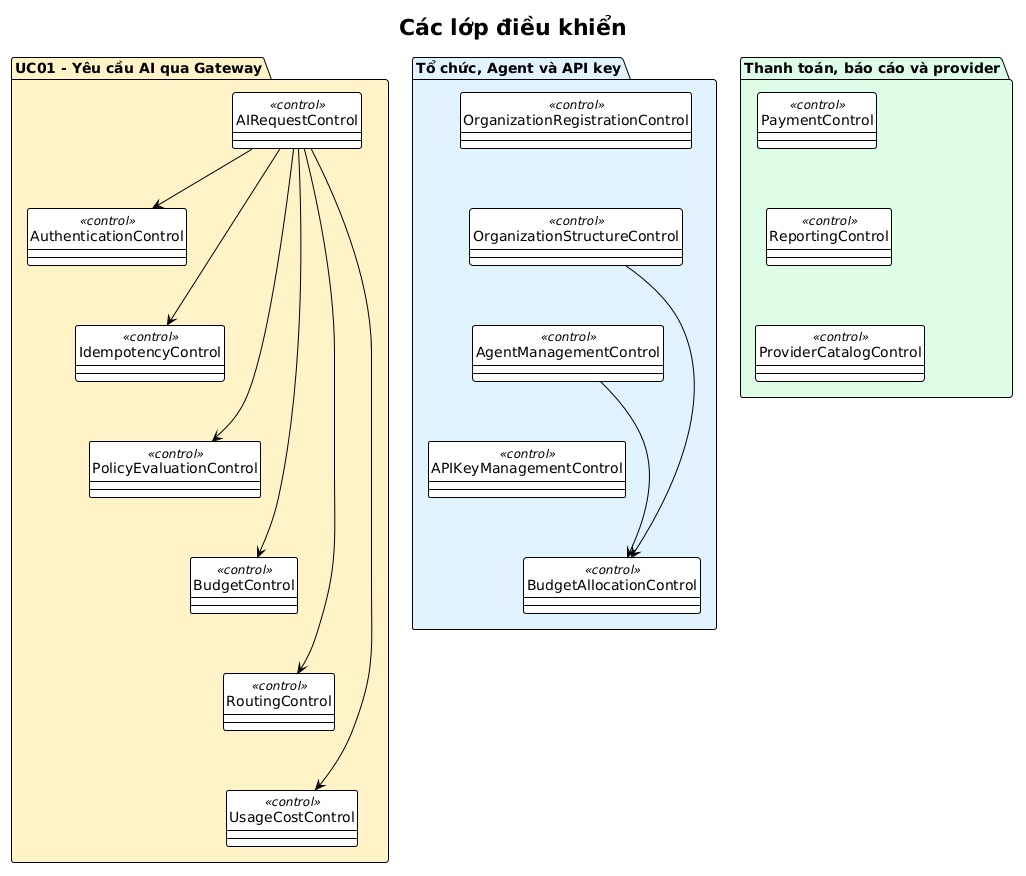
\includegraphics[width=0.96\textwidth,height=0.58\textheight,keepaspectratio]{report_support_documentation/diagrams/chapter_3/analysis_classes/sections/control.png}
    \caption[Biểu đồ lớp điều khiển]{Biểu đồ các lớp điều khiển theo nhóm trường hợp sử dụng}\label{fig:analysis-control-classes}
\end{figure}

\begin{longtable}{|L{0.29\textwidth}|L{0.61\textwidth}|}
\caption{Các lớp điều khiển trong mô hình phân tích}\\
\hline
\textbf{Lớp điều khiển} & \textbf{Trách nhiệm} \\
\hline
\endfirsthead
\hline
\textbf{Lớp điều khiển} & \textbf{Trách nhiệm} \\
\hline
\endhead
AIRequestControl & Điều phối toàn bộ UC01.\\
\hline
AuthenticationControl & Xác thực API key và xác định đường dẫn chịu chi phí.\\
\hline
IdempotencyControl & Nhận diện yêu cầu gửi lại và ngăn ghi nhận trùng.\\
\hline
\makecell[l]{PolicyEvaluation\\Control} & Kiểm tra trạng thái Agent, policy và quota.\\
\hline
BudgetControl & Kiểm tra ví tổ chức và hạn mức tại các cấp.\\
\hline
RoutingControl & Chọn provider, model và phương án thay thế.\\
\hline
UsageCostControl & Ghi nhận usage, cost, giao dịch và trace.\\
\hline
\makecell[l]{Organization\\Registration\\Control} & Tạo tổ chức, vai trò quản trị đầu tiên và ví tổ chức.\\
\hline
\makecell[l]{OrganizationStructure\\Control} & Quản lý đội ngũ, thành viên và quan hệ quản lý Agent.\\
\hline
\makecell[l]{AgentManagement\\Control} & Đăng ký, cập nhật trạng thái và bàn giao Agent.\\
\hline
\makecell[l]{APIKeyManagement\\Control} & Tạo, xem trạng thái và thu hồi API key của Agent.\\
\hline
\makecell[l]{BudgetAllocation\\Control} & Phân bổ hoặc thu hồi hạn mức giữa hai cấp liền kề.\\
\hline
PaymentControl & Xác thực top-up và cập nhật ví tổ chức.\\
\hline
ReportingControl & Truy xuất và tổng hợp dữ liệu theo phạm vi quyền.\\
\hline
ProviderCatalogControl & Quản lý provider, model, credential và chính sách giá.\\
\hline
\end{longtable}

Các lớp điều khiển chỉ điều phối nghiệp vụ. Trạng thái được lưu trong lớp thực thể.

\section{Phân tích lớp thực thể}

Lớp thực thể biểu diễn dữ liệu nghiệp vụ cần duy trì qua nhiều trường hợp sử dụng.

\begin{sidewaysfigure}[p]
    \centering
    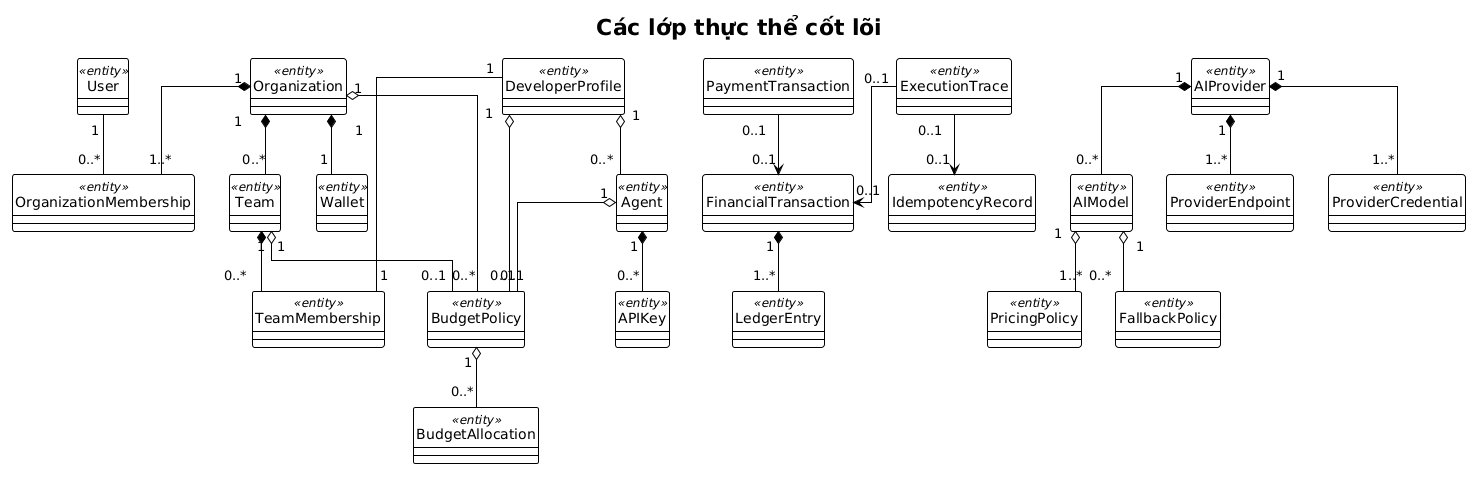
\includegraphics[width=0.94\textheight,height=0.86\textwidth,keepaspectratio]{report_support_documentation/diagrams/chapter_3/analysis_classes/sections/entity.png}
    \caption[Biểu đồ lớp thực thể]{Biểu đồ các lớp thực thể và quan hệ nghiệp vụ}\label{fig:analysis-entity-classes}
\end{sidewaysfigure}

\clearpage

\begin{longtable}{|L{0.27\textwidth}|L{0.63\textwidth}|}
\caption{Các lớp thực thể trong mô hình phân tích}\\
\hline
\textbf{Lớp thực thể} & \textbf{Ý nghĩa nghiệp vụ} \\
\hline
\endfirsthead
\hline
\textbf{Lớp thực thể} & \textbf{Ý nghĩa nghiệp vụ} \\
\hline
\endhead
User & Cá nhân có danh tính trong hệ thống.\\
\hline
Organization & Phạm vi sở hữu ví, đội ngũ, thành viên và Agent.\\
\hline
\makecell[l]{Organization\\Membership} & Vai trò của người dùng trong tổ chức.\\
\hline
Team & Cấp hạn mức giữa tổ chức và lập trình viên.\\
\hline
TeamMembership & Quan hệ giữa lập trình viên và đội ngũ.\\
\hline
DeveloperProfile & Hồ sơ lập trình viên quản lý Agent và hạn mức được cấp.\\
\hline
Agent & AI Agent bên ngoài được đăng ký vào Gateway.\\
\hline
APIKey & Khóa do Asymptotic cấp cho Agent.\\
\hline
Wallet & Số dư tiền của tổ chức.\\
\hline
BudgetPolicy & Hạn mức, quota và policy tại từng cấp.\\
\hline
BudgetAllocation & Lịch sử phân bổ hoặc thu hồi hạn mức.\\
\hline
FinancialTransaction & Giao dịch nạp tiền, sử dụng hoặc điều chỉnh tài chính.\\
\hline
LedgerEntry & Bút toán phục vụ truy vết và đối soát.\\
\hline
PaymentTransaction & Giao dịch nạp tiền với Payment Provider.\\
\hline
IdempotencyRecord & Khóa lũy đẳng và kết quả đã xử lý.\\
\hline
ExecutionTrace & Trạng thái, usage, cost và dấu vết của yêu cầu AI.\\
\hline
AIProvider & Nhà cung cấp dịch vụ AI.\\
\hline
AIModel & Mô hình do provider cung cấp.\\
\hline
ProviderEndpoint & Điểm cuối dùng để gọi provider.\\
\hline
ProviderCredential & Thông tin xác thực nội bộ của Gateway.\\
\hline
PricingPolicy & Biểu giá có hiệu lực của model.\\
\hline
FallbackPolicy & Quy tắc chọn provider hoặc model thay thế.\\
\hline
\end{longtable}

Chỉ \textit{Wallet} lưu tiền. Team, Developer và Agent được kiểm soát bằng \textit{BudgetPolicy}.

\section{Đối chiếu lớp phân tích với trường hợp sử dụng}

Robustness Diagram kiểm tra đường tương tác từ tác nhân qua lớp biên, lớp điều khiển đến lớp thực thể.

\begin{figure}[H]
    \centering
    
\includegraphics[width=\textwidth,height=0.72\textheight,keepaspectratio]{report_support_documentation/diagrams/chapter_3/robustness/UC01/diagram.png}
    \caption[Robustness Diagram UC01]{Robustness Diagram UC01 -- Thực hiện yêu cầu AI qua Gateway}\label{fig:robustness-uc01}
\end{figure}

\cref{fig:robustness-uc01} cho thấy AI Agent chỉ tương tác với lớp biên. Các kiểm tra xác thực, lũy đẳng, policy, ngân sách và định tuyến được điều phối trước khi ghi nhận kết quả.

\begin{figure}[H]
    \centering
    
\includegraphics[width=0.96\textwidth,height=0.62\textheight,keepaspectratio]{report_support_documentation/diagrams/chapter_3/robustness/UC04/diagram.png}
    \caption[Robustness Diagram UC04]{Robustness Diagram UC04 -- Đăng ký và quản lý AI Agent}\label{fig:robustness-uc04}
\end{figure}

\cref{fig:robustness-uc04} tách quản lý Agent khỏi quản lý API key và phân bổ hạn mức. UC04 chỉ quản lý thông tin, trạng thái và người phụ trách Agent.

{\footnotesize
\begin{longtable}{|L{0.06\textwidth}|L{0.23\textwidth}|L{0.29\textwidth}|L{0.27\textwidth}|}
\caption{Đối chiếu trường hợp sử dụng với lớp phân tích}\\
\hline
\textbf{UC} & \textbf{Lớp biên} & \textbf{Lớp điều khiển} & \textbf{Lớp thực thể chính} \\
\hline
\endfirsthead
\hline
\textbf{UC} & \textbf{Lớp biên} & \textbf{Lớp điều khiển} & \textbf{Lớp thực thể chính} \\
\hline
\endhead
UC01 & \makecell[l]{GatewayRequest\\Boundary,\\AIProviderBoundary} & AIRequestControl,\newline AuthenticationControl,\newline IdempotencyControl,\newline PolicyEvaluationControl,\newline BudgetControl,\newline RoutingControl,\newline UsageCostControl & Agent, APIKey,\newline Wallet, BudgetPolicy,\newline IdempotencyRecord,\newline AIProvider, AIModel,\newline FinancialTransaction,\newline ExecutionTrace\\
\hline
UC02 & \makecell[l]{OrganizationBoundary,\\PaymentProvider\\Boundary} & PaymentControl & Organization, Wallet,\newline PaymentTransaction,\newline FinancialTransaction,\newline LedgerEntry\\
\hline
UC03 & OrganizationBoundary & BudgetAllocationControl,\newline BudgetControl & Organization, Team,\newline DeveloperProfile, Agent,\newline Wallet, BudgetPolicy,\newline BudgetAllocation\\
\hline
UC04 & OrganizationBoundary & AgentManagementControl,\newline OrganizationStructureControl & Organization, Team,\newline DeveloperProfile, Agent\\
\hline
UC05 & OrganizationBoundary & APIKeyManagementControl & Organization,\newline DeveloperProfile,\newline Agent, APIKey\\
\hline
UC06 & ReportingBoundary & ReportingControl & Organization, Team,\newline DeveloperProfile, Agent,\newline FinancialTransaction,\newline LedgerEntry, ExecutionTrace\\
\hline
UC07 & \makecell[l]{OrganizationRegistration\\Boundary} & \makecell[l]{OrganizationRegistration\\Control} & User,\newline Organization,\newline OrganizationMembership,\newline Wallet\\
\hline
UC08 & OrganizationBoundary & OrganizationStructureControl,\newline AgentManagementControl,\newline BudgetAllocationControl & User, Organization,\newline OrganizationMembership,\newline Team, TeamMembership,\newline DeveloperProfile, Agent,\newline BudgetPolicy\\
\hline
UC09 & SystemAdminBoundary & ProviderCatalogControl & AIProvider, AIModel,\newline ProviderEndpoint,\newline ProviderCredential,\newline PricingPolicy,\newline FallbackPolicy\\
\hline
\end{longtable}
}

Bảng đối chiếu bảo đảm mỗi trường hợp sử dụng có điểm tương tác, trách nhiệm điều phối và trạng thái nghiệp vụ tương ứng. Đây là đầu vào cho thiết kế lớp và tương tác ở Chương 4.

\section*{Kết luận chương}

Chương này đã xác định các lớp Boundary--Control--Entity và truy vết chúng về UC01--UC09. Mô hình là cơ sở cho thiết kế gói, lớp, tương tác, trạng thái và dữ liệu ở Chương 4.
